%%%%%%%%%%%%%%%%%%%%%%%%%%%%%%%%%%%%%%%%%
% NIWeek 2014 Poster by T. Reveyrand
% www.microwave.fr
% http://www.microwave.fr/LaTeX.html
% ---------------------------------------
% 
% Original template created by:
% Brian Amberg (baposter@brian-amberg.de)
%
% This template has been downloaded from:
% http://www.LaTeXTemplates.com
%
% License:
% CC BY-NC-SA 3.0 (http://creativecommons.org/licenses/by-nc-sa/3.0/)
%
%%%%%%%%%%%%%%%%%%%%%%%%%%%%%%%%%%%%%%%%%

%----------------------------------------------------------------------------------------
%	PACKAGES AND OTHER DOCUMENT CONFIGURATIONS
%----------------------------------------------------------------------------------------

\documentclass[a0paper,portrait]{baposter}

\usepackage[font=small,labelfont=bf]{caption} % Required for specifying captions to tables and figures
\usepackage{booktabs} % Horizontal rules in tables
\usepackage{relsize} % Used for making text smaller in some places

\usepackage{amsmath,amsfonts,amssymb,amsthm} % Math packages
\usepackage{eqparbox}

\usepackage{textcomp}

\usepackage{wrapfig}

\usepackage{picinpar}

\usepackage{picins}

\graphicspath{{figures/}} % Directory in which figures are stored

 \definecolor{bordercol}{RGB}{40,40,40} % Border color of content boxes
 \definecolor{headercol1}{RGB}{186,215,230} % Background color for the header in the content boxes (left side)
 \definecolor{headercol2}{RGB}{120,120,120} % Background color for the header in the content boxes (right side)
 \definecolor{headerfontcol}{RGB}{0,0,0} % Text color for the header text in the content boxes
 \definecolor{boxcolor}{RGB}{210,235,250} % Background color for the content in the content boxes


\begin{document}

\background{ % Set the background to an image (background.pdf)
\begin{tikzpicture}[remember picture,overlay]
\draw (current page.north west)+(-2em,2em) node[anchor=north west]
{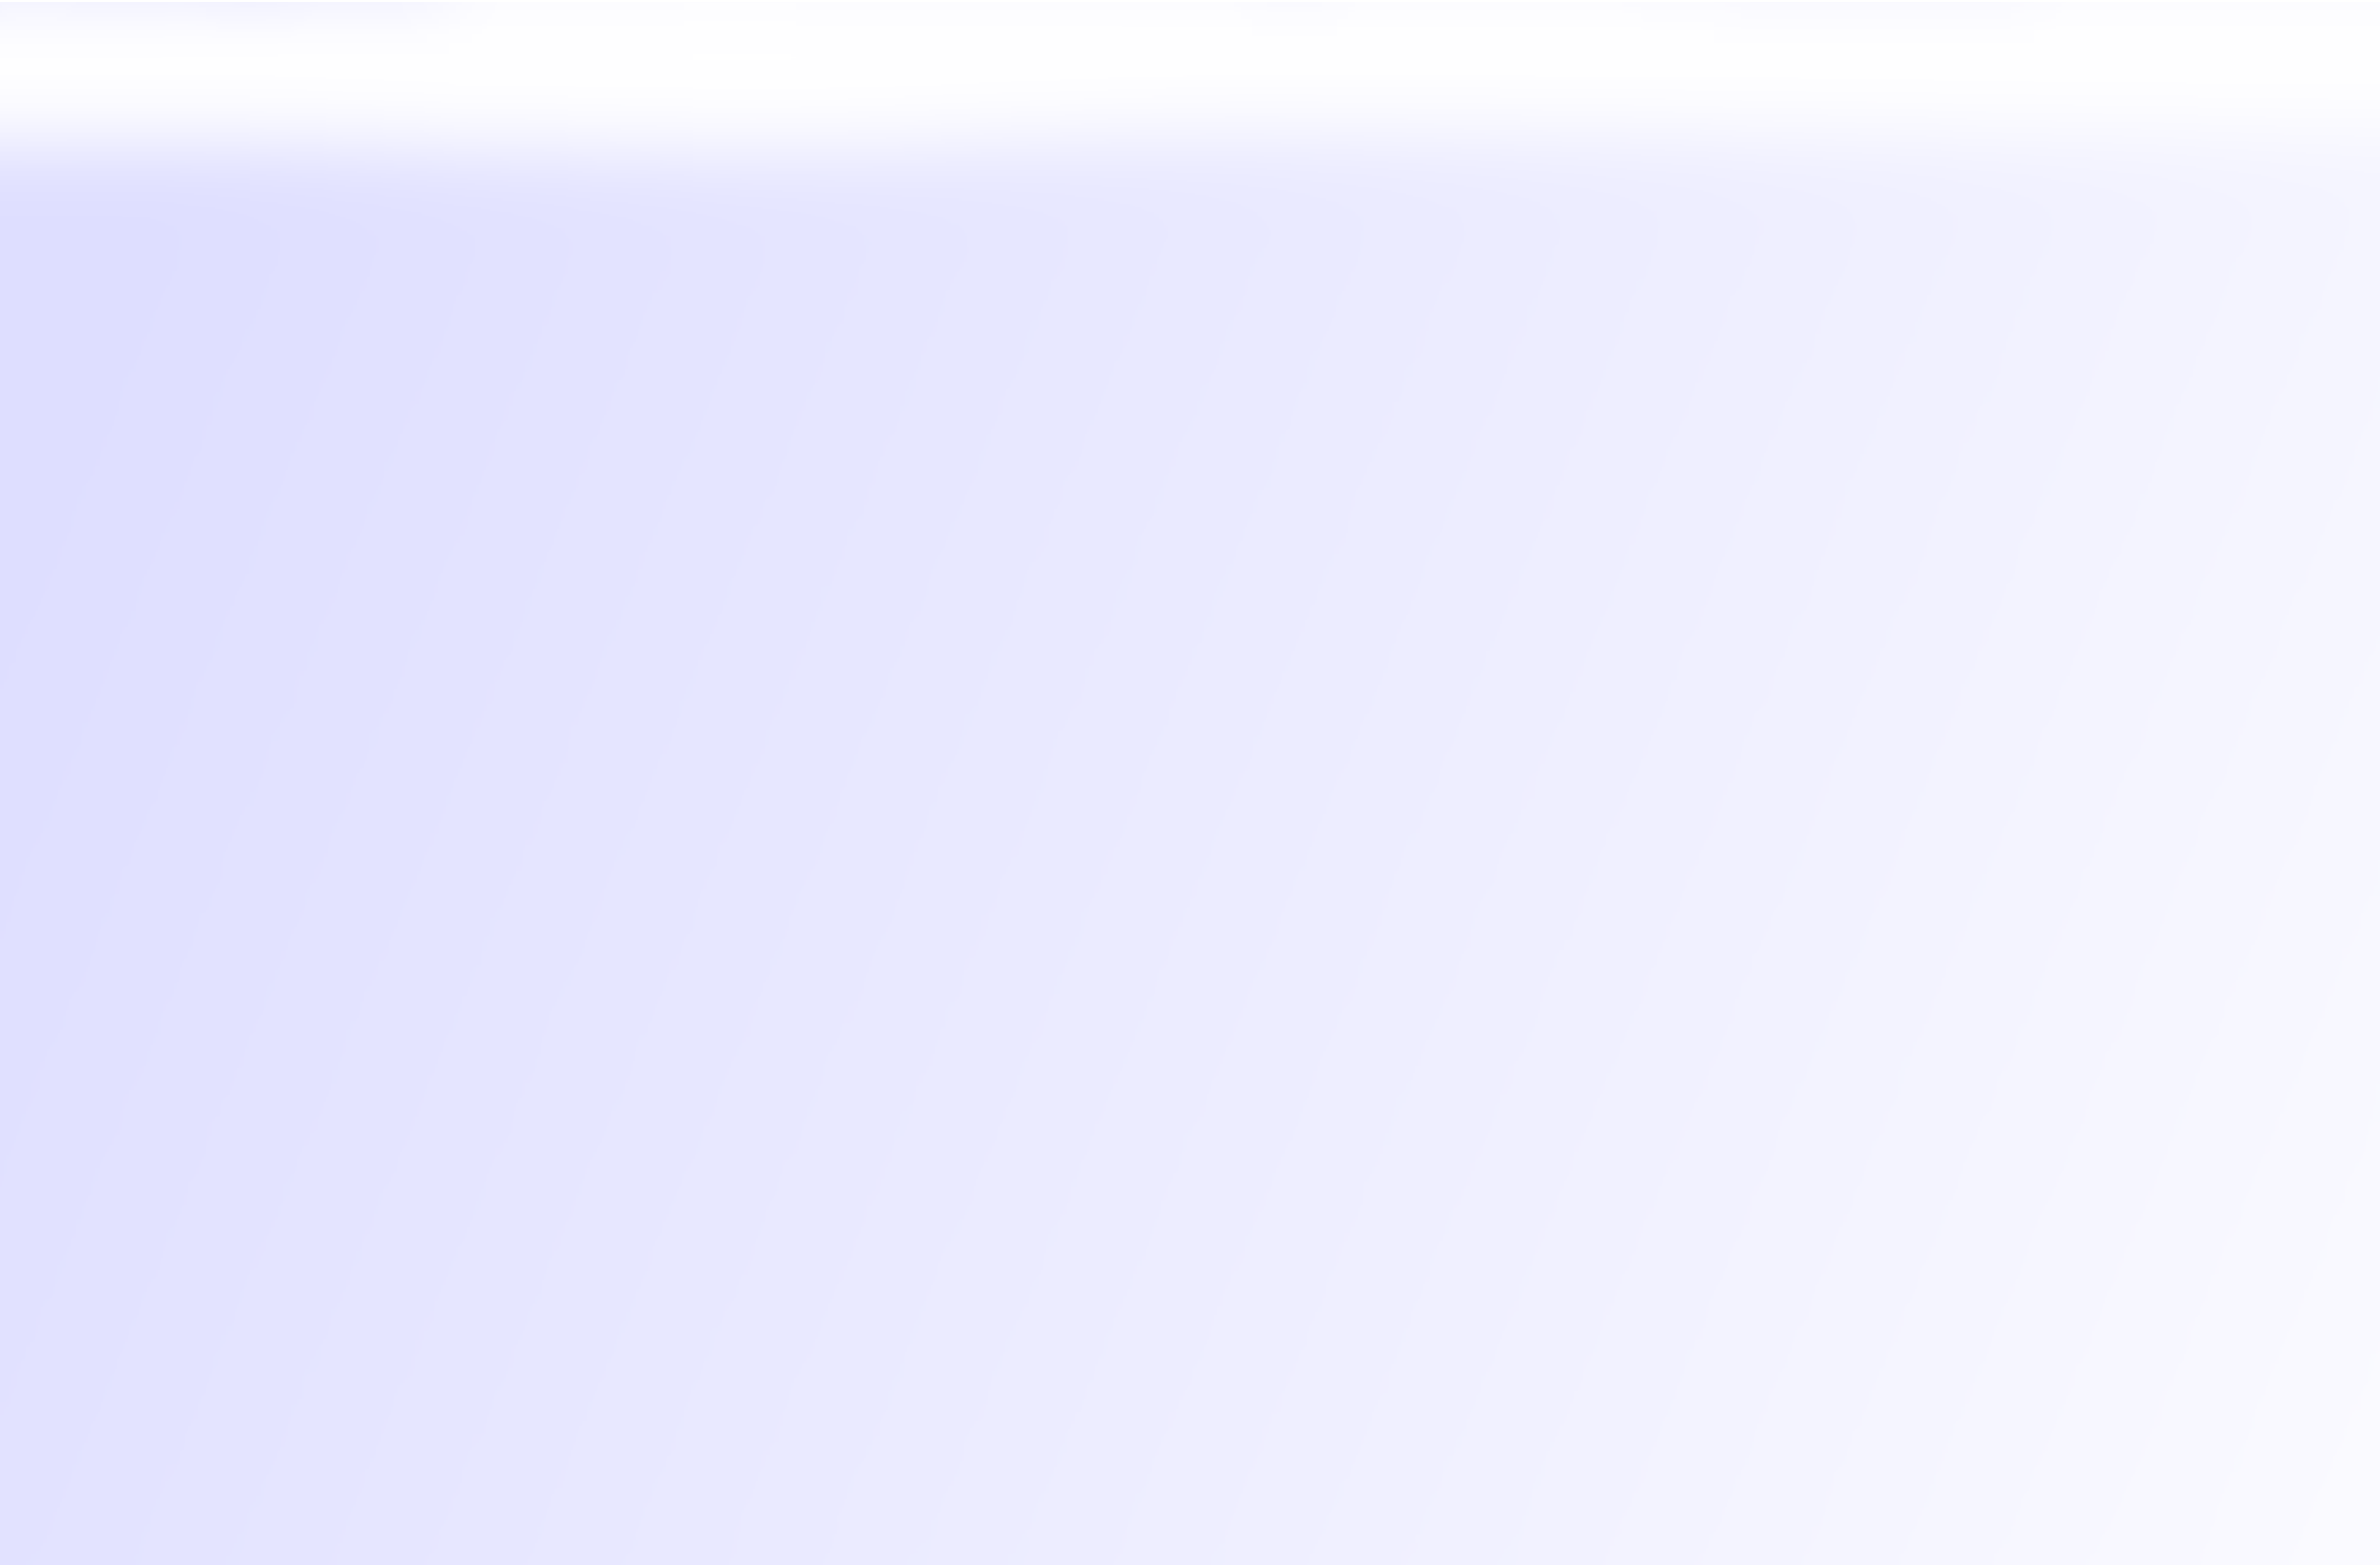
\includegraphics[height=1.1\textheight]{background}};
\end{tikzpicture}
}

\begin{poster}{
grid=false,
borderColor=bordercol, % Border color of content boxes
headerColorOne=headercol1, % Background color for the header in the content boxes (left side)
headerColorTwo=headercol2, % Background color for the header in the content boxes (right side)
headerFontColor=headerfontcol, % Text color for the header text in the content boxes
boxColorOne=boxcolor, % Background color for the content in the content boxes
headershape=roundedright, % Specify the rounded corner in the content box headers
headerfont=\Large\sf\bf, % Font modifiers for the text in the content box headers
textborder=rectangle,
background=user,
headerborder=open, % Change to closed for a line under the content box headers
boxshade=plain
}
{
\includegraphics[scale=0.3]{CEPCLogo.jpg}}
%
%----------------------------------------------------------------------------------------
%	TITLE AND AUTHOR NAME
%----------------------------------------------------------------------------------------
%
{ \bf  \huge {Status of design and development of CEPC-DHCAL readout electronics} } % Poster title
{\vspace{0.3em} \smaller Yu Wang$^{1,2}$, Daojin Hong$^{1,2}$, Jianbei Liu$^{1,2}$, Shubin Liu$^{1,2}$, Changqing Feng\'c$^{1,2}$, Yi Zhou$^{1,2}$   \\  % Author names
  
\smaller $^1$\it {University of Science and Technology of China} \\ $^2$\it{State Key Laboratory of Particle Detection and Electronics} } % Author email addresses
{
\includegraphics[scale=0.2]{ustcblue.jpg}} % University/lab logo

%----------------------------------------------------------------------------------------
%	INTRODUCTION
%----------------------------------------------------------------------------------------
\headerbox{Introduction}{name=introduction,column=0,row=0, span=3}{
\begin{itemize} 
	\item The goal of this research is to provide a feasible readout scheme for CEPC DHCAl. 
	\vspace{-0.2cm}
	\item As the active detector element of sampling calorimeter has finely segmented readout pads of $1\times1cm^2$, it's a real challenge to access huge mount data from calorimeter.
	\vspace{-0.2cm}
	%\item In PFA-based calorimeters, simulation results suggest that for readout segments as small as $1cm^2$, simple hit counting is already a good energy measurement for hadrons, so called DHCAL. A more general calorimeter with multi-threshold readout (e.g. 3 thresholds) records more detailed hit information and has better energy for jet energy above 40GeV, a so-called Semi-Digital Hadron Calorimeter (SDHCAL)
	%\vspace{-0.2cm}
	\item In our research, a double layer GEM using self-stretching technique has been used. It consists of 3mm drift gap, 1mm transfer gap and 1mm induction gap and the effective area is $30\times30cm^2$with $1\times1cm^2$ readout pads.
	\vspace{-0.2cm}
	\item The chip choosen to readout is a tri-thresholds ASIC called MICROROC (MICRO-mesh gaseous structure Read-Out Chip)
\end{itemize}
}


%----------------------------------------------------------------------------------------
%	CALIBRATION
%----------------------------------------------------------------------------------------

\headerbox{MICROROC ASIC}{name=Microroc,column=0,below=introduction}{
MICROROC is a 64-channel Semi-Digital readout chip, developed at IN2P3 by OMEGA/LAL. The package of MICROROC chip is TQFP which means the thickness is about 1.4mm. %The flowing picture shows the MICROROC chip.
\vspace{-0.2cm}
%\begin{center}
%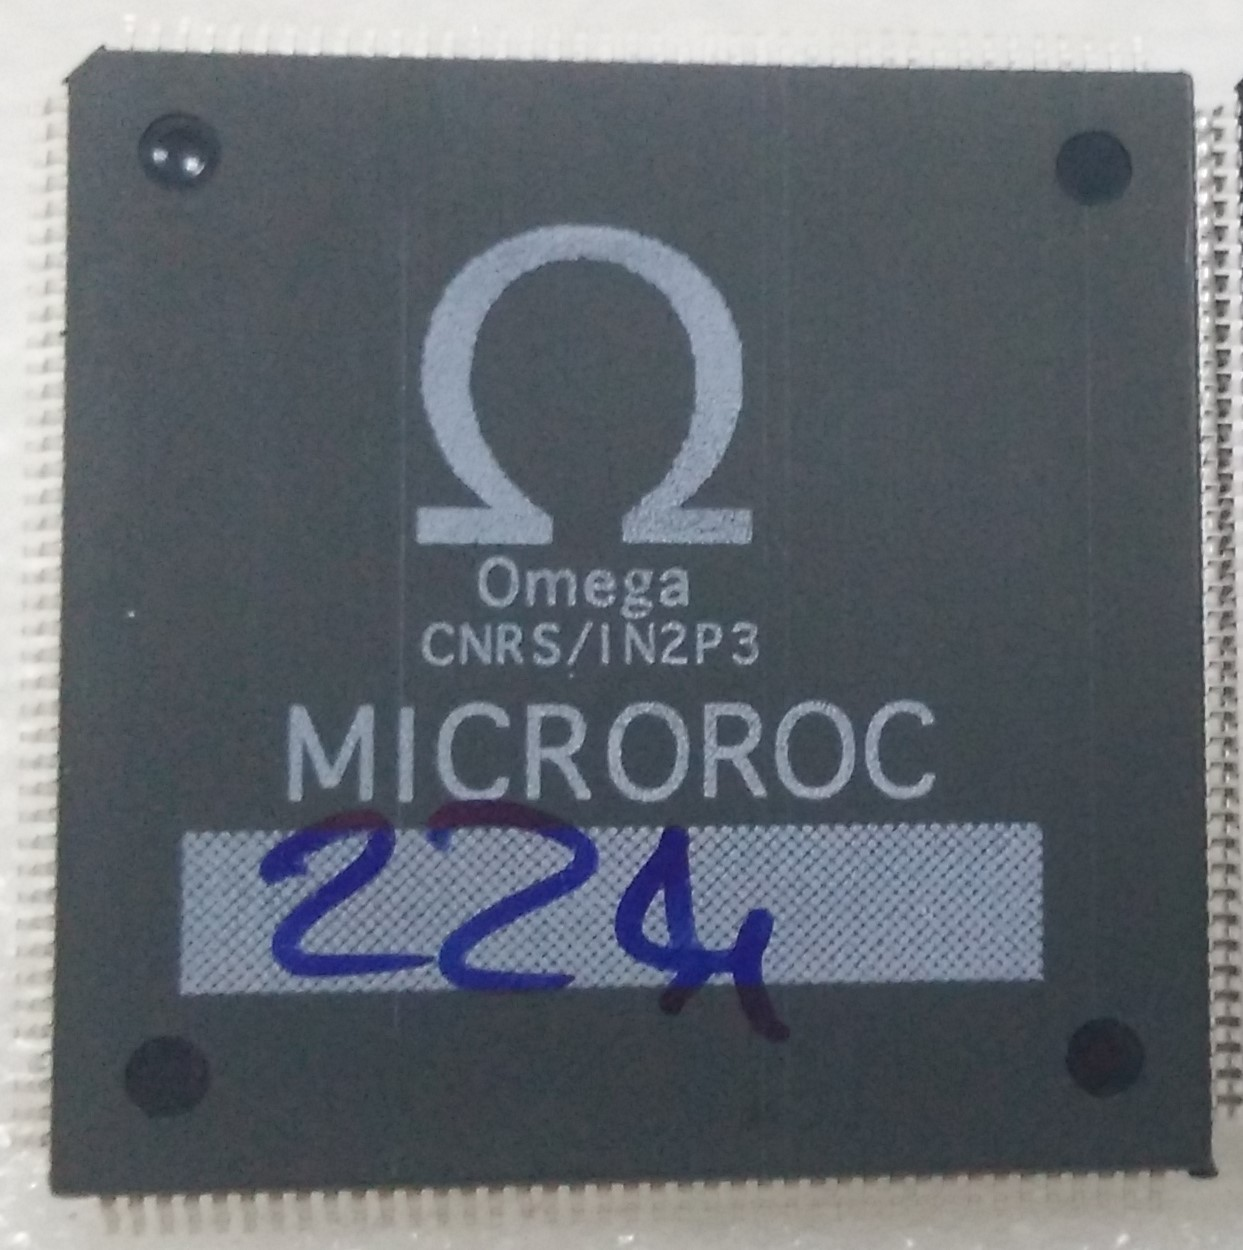
\includegraphics[scale=0.08]{figures/MicrorocChip.jpg}
%\end{center}
Each channel of the MICROROC chip has:
\begin{itemize}
	\item A very low noise charge preamplifier, able to handle a dynamic range from 1 fC to 500fC
	\vspace{-0.3cm}
	\item Two different adjustable shaper. A high gain shaper for small signal and a low gain shaper for large signal
	\vspace{-0.3cm}
	\item Three comparators for tri-thresholds readout
	\vspace{-0.3cm}
	\item A random access memory used as a digital buffer
\end{itemize}
The structure of the analog part is shown below:
\begin{center}
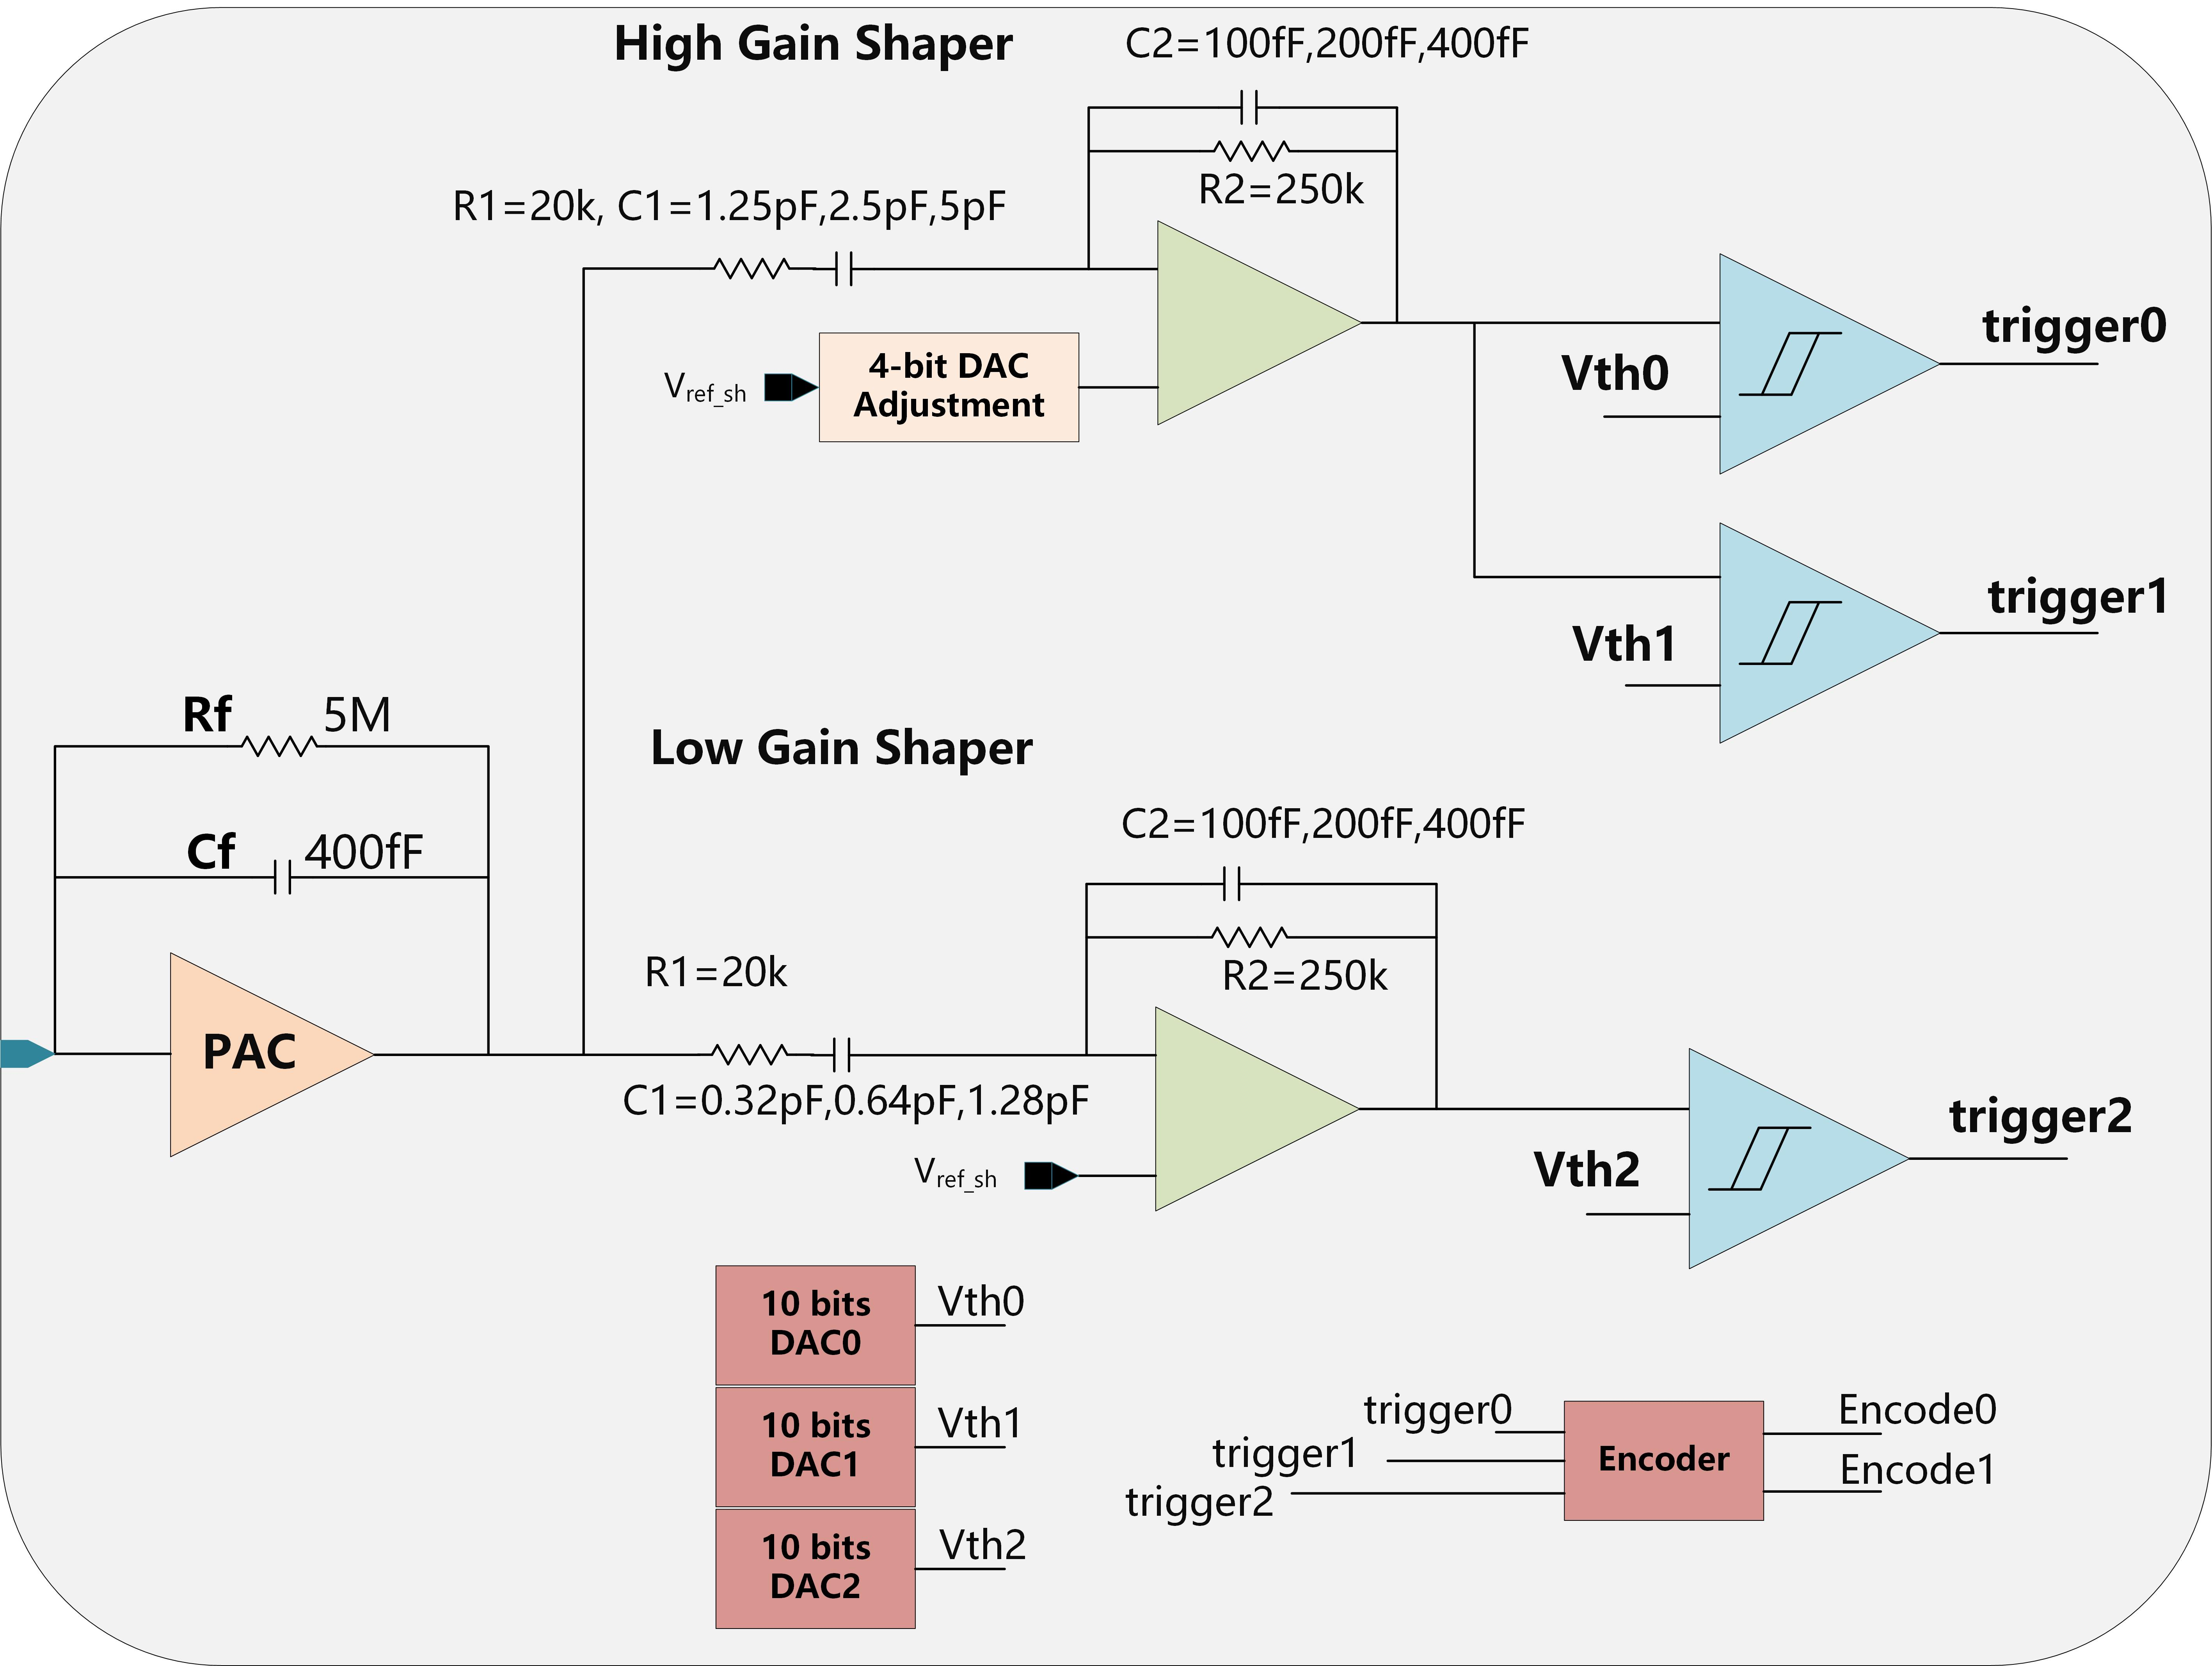
\includegraphics[scale=0.3]{figures/MicrorocStructureTransparent.png}
\end{center}
}
\headerbox{GEM Detector}{name=GEM,column=0,below=Microroc}{

\begin{tikzpicture}
\draw (0em,0em) node(ImageGEMHole)[anchor=west]{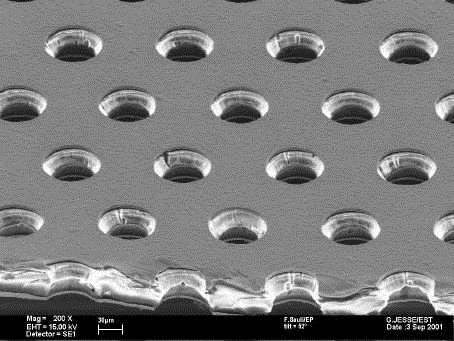
\includegraphics[width=.4\textwidth]{figures/GEMHole.jpg}};%
\draw (ImageGEMHole.east) node(TextSelfStretch)[anchor=west]{
\begin{minipage}{0.6\textwidth}
	\begin{enumerate}
	\item Cu:t = 5$\mu$m
	\vspace{-0.3cm}
	\item Kapton:T = 50$\mu$m
	\vspace{-0.3cm}
	\item Diameter: d = 60$\mu$m
	\vspace{-0.3cm}
	\item D = 80$\mu$m
	\vspace{-0.3cm}
	\item pitch: 140$\mu$m
	\end{enumerate}
\end{minipage}
};
\draw[thick] (ImageGEMHole.south west) ++(0em,-1em) -- ++(20.5em,0em);
\draw (ImageGEMHole.south) +(0em,-3.5em) node(ImageSelfStretch)[anchor=north]{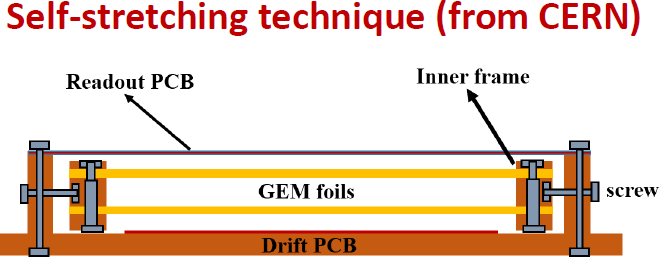
\includegraphics[width=0.4\textwidth]{figures/SelfStreching.png}};
\draw (ImageSelfStretch.east) node(TextSelfStretch)[anchor=west]{
\begin{minipage}{0.6\textwidth}
\begin{enumerate}
\item Assembling process is easy and fast
\vspace{-0.3cm}
\item No dead area inside the active area
\vspace{-0.3cm}
\item Uniform gas flow
\vspace{-0.3cm}
\item Detachable
\end{enumerate}
\end{minipage}
};
\draw[thick] (ImageSelfStretch.south west) ++(0em,-2.5em) -- ++(20.5em,0em);
\draw (ImageSelfStretch.south) +(1em,-3.5em) node(ImageGEMDetector)[anchor=north]{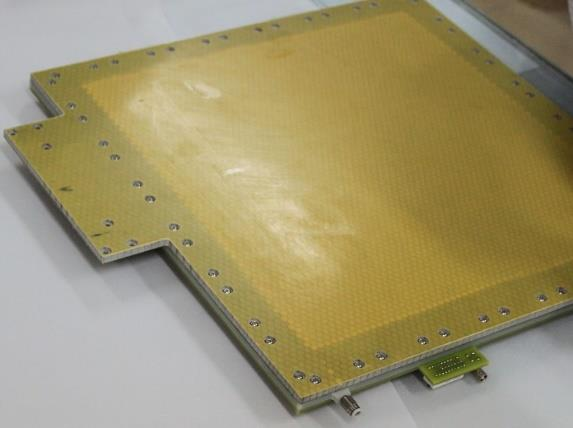
\includegraphics[height=0.3\textwidth]{figures/GEMDetector.jpg}};
\draw (ImageGEMDetector.east) +(1em,0em) node(ImageStructureOfGEM)[anchor=west]{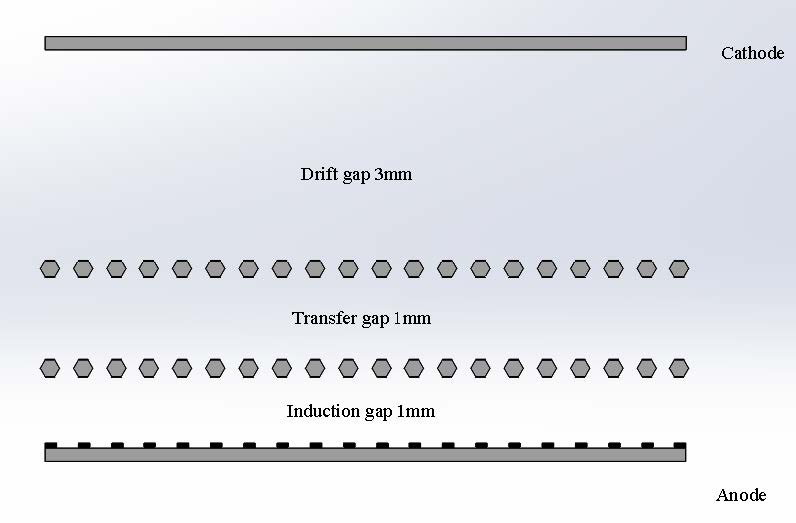
\includegraphics[height=0.3\textwidth]{figures/StructureOfGEM.jpg}};
\end{tikzpicture}
}


%----------------------------------------------------------------------------------------
%	OTHER INSTRUMENTATION
%----------------------------------------------------------------------------------------
\headerbox{Readout System Structure}{name=ReadoutSystemStructure,span=2,column=1,row=1, below=introduction}{ % To reduce this block to 1 column width, remove 'span=2'
The readout system is developed on SRS(Scalable Readout System), which means users can reuse the same system just changing the front-end board.The whole system includes flowing parts:
\begin{itemize}
	\item FEB(Front-End Board):Combination of detector and readout ASIC
	\vspace{-0.2cm}
	\item DIF(Detector InterFace):Control the ASIC and read back data
	\vspace{-0.2cm}
	\item DAQ:Distribute clock and command. Gather data from DIF
\end{itemize}
The system structure of the hole system is shown below
\begin{center}
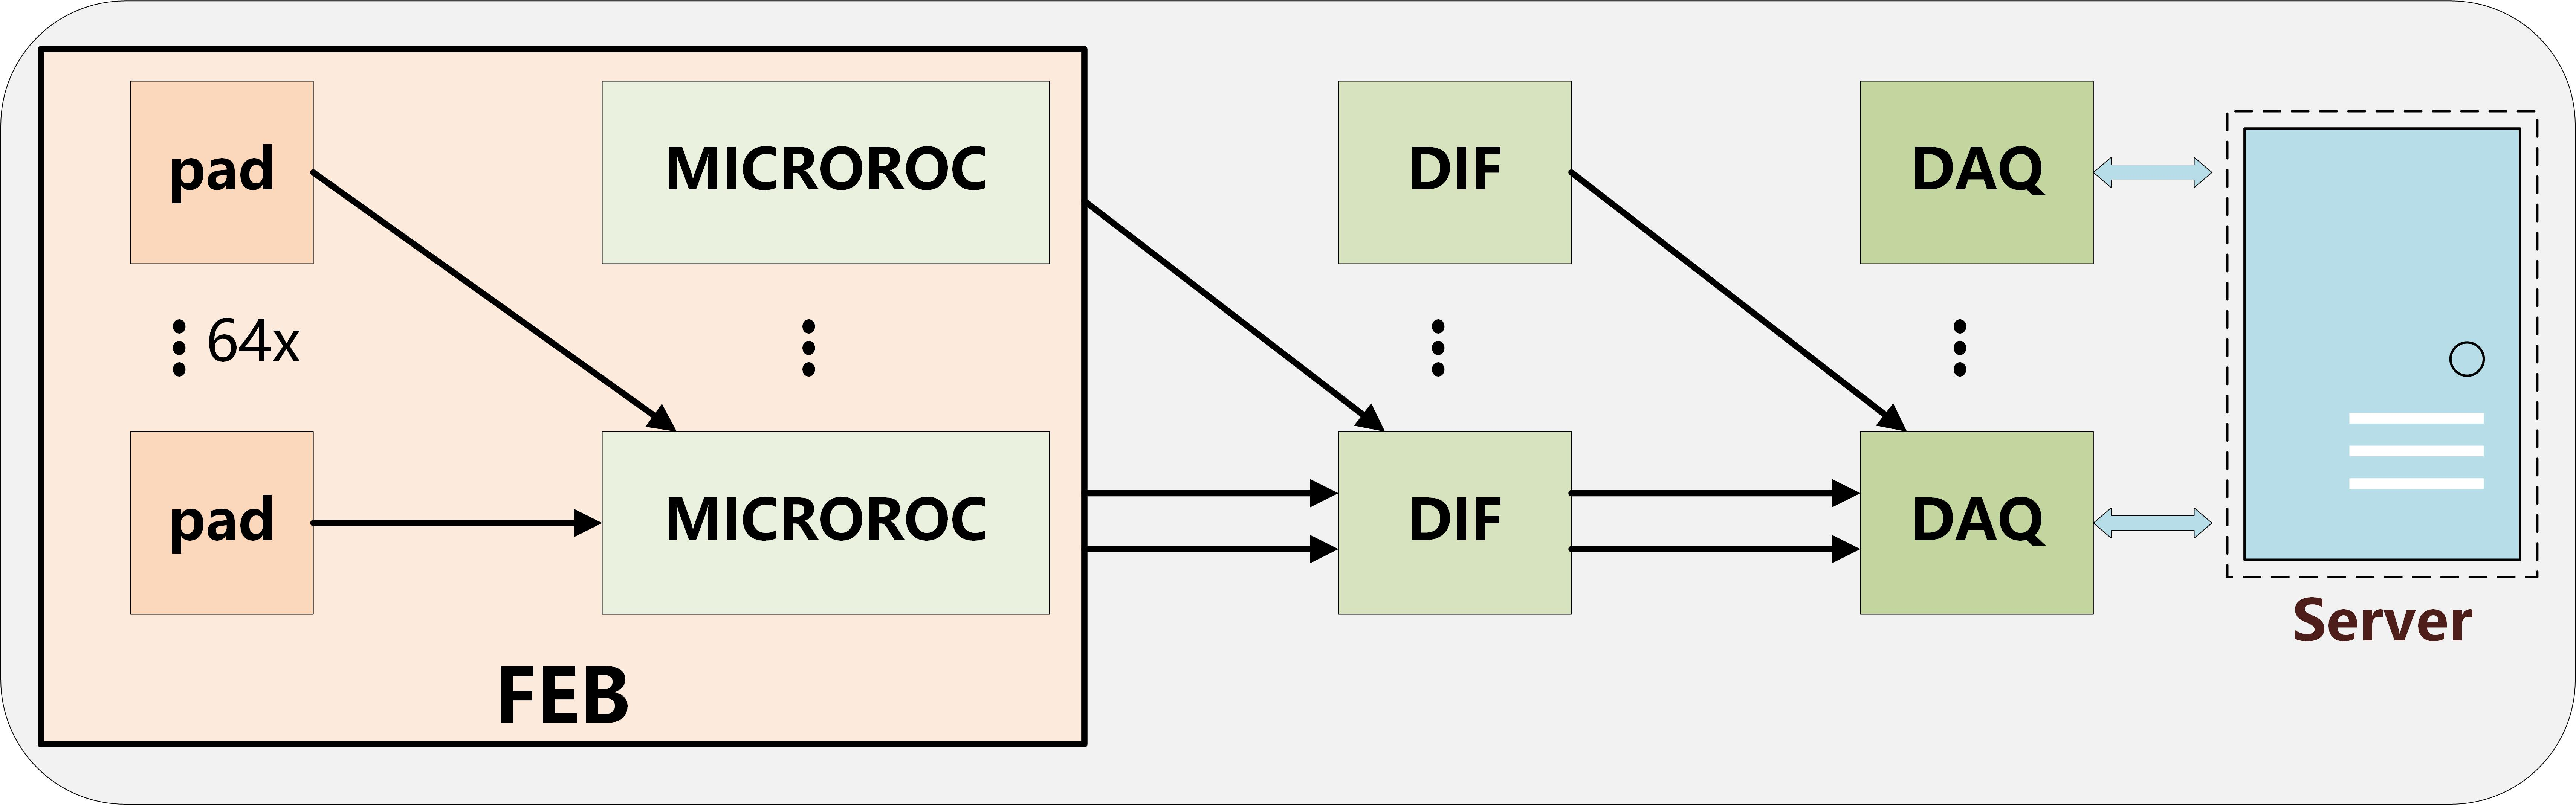
\includegraphics[scale=0.6]{figures/ReadoutStructureTransparent.png}
\end{center}

}


%----------------------------------------------------------------------------------------
%	MIXER vs. SAMPLERS
%----------------------------------------------------------------------------------------
\headerbox{Phase I Design and Test}{name=FirstStageDesignAndTest,span=2,column=1,row=1, below=ReadoutSystemStructure}{
A "Phase I" design is completed to verify the readout structure and test the performance of MICROROC. The front-end ASIC is separated from the detector plane. The system shown below contains the GEM detector, FEB and DIF.\\
\vspace{-0.5cm}
\begin{center}
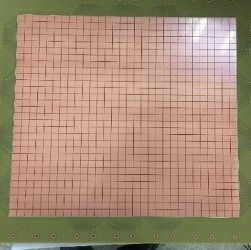
\includegraphics[height=2.5cm]{figures/ReadOutPlane.jpg} 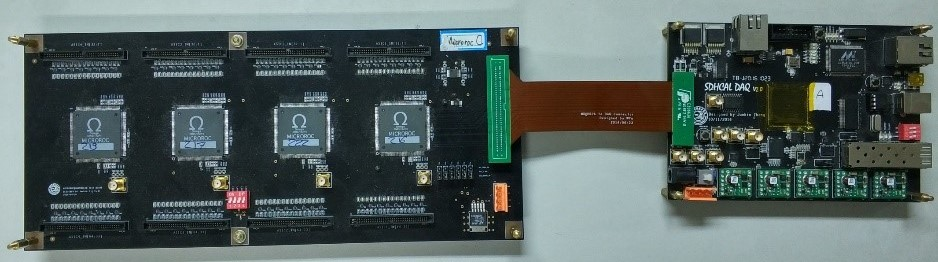
\includegraphics[height=2.5cm]{figures/PhaseIDesign.jpg}
\end{center}

}



%----------------------------------------------------------------------------------------
%	MEASUREMENT SETUP
%----------------------------------------------------------------------------------------
\headerbox{Next Step}{name=NextStep,span=2,column=1,below=FirstStageDesignAndTest}{ 

}


%----------------------------------------------------------------------------------------
%	CONCLUSION
%----------------------------------------------------------------------------------------
\headerbox{Conclusion}{name=conclusion,column=1,below=NextStep,span=2}{
Total Conclusion
\vspace{-0.2cm}
\begin{itemize} 
\item d
\vspace{-0.2cm}
\item c
\vspace{-0.2cm}
\item b
\vspace{-0.2cm}
\item a
\item d
\vspace{-0.2cm}
\item c
\vspace{-0.2cm}
\item b
\vspace{-0.2cm}
\item a


\end{itemize}
}


%----------------------------------------------------------------------------------------
%	REFERENCES
%----------------------------------------------------------------------------------------

%\headerbox{References}{name=references,column=2,below=application}{

%\smaller % Reduce the font size in this block
%\renewcommand{\section}[2]{\vskip 0.05em} % Get rid of the default "References" section title
%\nocite{*} % Insert publications even if they are not cited in the poster

%\bibliographystyle{unsrt}
%\bibliographystyle{IEEEtran}
%\bibliography{biblio} % Use biblio.bib as the bibliography file
%}


%----------------------------------------------------------------------------------------
%	ACKNOWLEDGEMENTS
%----------------------------------------------------------------------------------------

\headerbox{Acknowledgements}{name=acknowledgements,column=0,below=GEM, above=bottom,span=3}{
\smaller 
This study was supported by National Key Programme for S\&T Research and Development (Grant NO.: 2016YFA0400400). Thanks to St\'ephane CALLIER and Christophe de LA TAILLE at OMEGA - IN2P3/CNRS for helpful discussions and useful suggestions
} 


Auther email:wyu0725@mail.ustc.edu.cn
\end{poster}

\end{document}